\begin{frame}
	\frametitle{Poder de Mercado}
	Em geral, \'e a capacidade de uma empresa influenciar o pre\c co de venda do seu produto, bem como o pre\c copraticado pelas empresas concorrentes em mercados oligopolistas, atrav\'es de:
	\begin{itemize}
		\item Manipula\c c\~ao da vari\'avel estrat\'egica:
		\begin{itemize}
			\item Pre\c co
			\item Quantidade
		\end{itemize}
	\end{itemize}
\end{frame}

\begin{frame}
	\frametitle{Poder de Mercado}
	Fontes do poder de mercado:
	\begin{itemize}
		{\footnotesize
		\item Empresas instaladas em mercados com Barreiras \`a Entrada (barreiras naturais e barreiras legais);
		\item Empresas instaladas em nichos de mercado, explorando uma procura fiel ou fidelizada, enfrentando pouca concorr\^encia (bens sem substitutos);
		\item Diferencia\c c\~ao do prodto; cria\c c\~ao de procura fidelizada;
		\item Custos de transporte; custos de mudan\c ca; custos de busca de informa\c c\~ao
		}
	\end{itemize}
\end{frame}

\begin{frame}
	\frametitle{Discrimina\c c\~ao de Pre\c cos}
	Pr\'atica que consiste em fixar pre\c cos diferenttes para o mesmo produto, em fun\c c\~ao da quantidade comprada e/ou da disponibilidade a pagar do consumidor, em situa\c c\~oes em que as empresas t\^en \textbf{\underline{poder de mercado}}\par
	\vspace{0.5cm}
	A discrimina\c c\~ao ocorre quando uma empresa cobra pre\c cos diferentes:
	\begin{itemize}
		\item para cada unidade do bem, em fun\c c\~ao do pre\c co de reserva, ou seja, da disponibilidade a pagar, de cada consumidor (1\textsuperscript{\underline{o}} grau)
		\item para escal\~oes diferentes de consumo (2\textsuperscript{\underline{o}} grau)
		\item para grupos de consumidores ou mercados distintos (3\textsuperscript{\underline{o}} grau)
	\end{itemize}
\end{frame}

\begin{frame}
	\frametitle{Cond\c c\~oes para que a discrimina\c c\~ao de pre\c cos seja vi\'avel}
	\begin{itemize}
		\setlength{\itemsep}{1.2em}
		\item O vendedor tem que ser capaz de identificar os diferentes consumidores
		\item N\~ao pode existir revenda (comprar mais barato para vender mais caro)
	\end{itemize}
\end{frame}

\begin{frame}
	\frametitle{A Discrimina\c c\~ao Perfeita (1\textsuperscript{\underline{o}} Grau)}
	\begin{itemize}
		\setlength{\itemsep}{1.5em}
		\item O monopolista cobra o pre\c co mais alto que cada consumidor est\'a disposto a pagar (pre\c co de reserva).
		\item A Procura coincide com a curva da receita marginal. O excedente do consumidor anula-se...
		\item A produ\c c\~ao total \'e igual \`a que se obt\'em em concorr\^encia perfeita, vejamos...
	\end{itemize}
\end{frame}

\begin{frame}
	\frametitle{A Discrimina\c c\~ao Perfeita (1\textsuperscript{\underline{o}} Grau)}
	Caso em que o $Cmg$ \'e constante
	\begin{columns}
		\begin{column}{0.47\textwidth}
			\begin{center}
				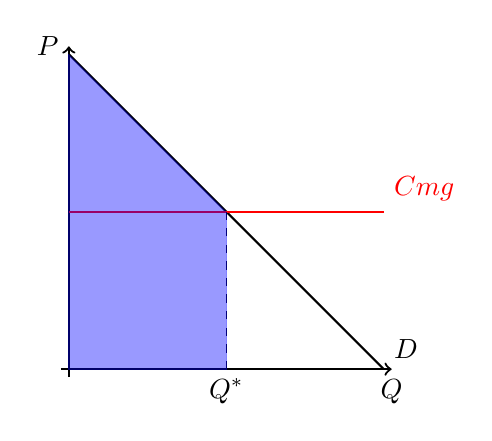
\begin{tikzpicture}[
					declare function = {
						d(\x) = 4-\x;
						cmg(\x) = 2;
					}]
					\draw[thick,->] (-0.1,0) -- (4.1,0)node[below]{$Q$};
					\draw[thick,->] (0,-0.1) -- (0,4.1)node[left]{$P$};

					\draw[domain=0:4,variable=\x,thick] plot (\x,{d(\x)})node[above right]{$D$};
					\draw[domain=0:4,variable=\x,red,thick] plot (\x,{cmg(\x)})node[above right]{$Cmg$};

					\draw[dashed] (2,0)node[below]{$Q^*$} -- (2,{d(2)});

					\onslide<2->{
						\draw[fill,blue,opacity=0.4] (0,4) -- (0,0) -- (2,0) -- (2,2);
					}
				\end{tikzpicture}
			\end{center}
		\end{column}
		\begin{column}{0.47\textwidth}
			\begin{itemize}
				{\footnotesize
				\item $Rmg=P$,  j\'a que o produtor cobra o pre\c co de reserva, i.e., o m\'aximo que o consumidor est\'a disposto a pagar...
				\item Ent\~ao a quantidade \'optima ocorre quando $Cmg=P$
				\item Do ponto de vista de efici\^encia, esta situa\c c\~ao \'e id\^entica \`a de concorr\^encia perfeita, mas do ponto de vista de quidade \'e contr\'aria... porqu\^e?
				\item A \'area sobreada coincide com a receita do produtor. O excedente que seria do consumidor \'e, agora, do produtor...
				}
			\end{itemize}
		\end{column}
	\end{columns}
\end{frame}

\begin{frame}
	\frametitle{A Discrimina\c de pre\c cos de 2\textsuperscript{\underline{o}} Grau}
	\begin{itemize}
		\setlength{\itemsep}{1.5em}
		\item O produtor cobra pre\c cos diferentes para escal\~oes diferentes de consumo de um bem ou servi\c co (venda por \emph{blocos})
		\item Aplica-se essencialmente quando os custos marginais s\~ao constantes
		\item \'E o caso dos descontos de quantidade...
	\end{itemize}
\end{frame}

\begin{frame}
	\frametitle{A discrimina\c do 3\textsuperscript{\underline{o}} Grau}
	\begin{itemize}
		\setlength{\itemsep}{1.5em}
		\item O produtor cobra pre\c cos diferentes a consumidores diferentes (ou em mercados diferentes). Realiza, deste modo, uma segmenta\c c\~ao do mercado aproveeitando a exist\^encia de pre\c cos de reserva distintos.
		\item Exemplos:
		\begin{itemize}
			\item descontos a estudantes ou a idosos
			\item produtos vendidos em mercados diferentes ou segmentos de mercado diferentes
		\end{itemize}
		\item \emph{O objectivo \'e sempre o mesmo: transformar excedente de consumidor em receita...\'e uma forma de exerc\'icio de poder de mercado}
	\end{itemize}
\end{frame}